\section{Data}
The following will include an overview and visualisation of the data acquired for the research, and how it was processed.

\subsection{\ac{ehm} Data}
The majority of data used for the research is \ac{ehm} data. This data was recorded by sensors in 231 BR725 engines during a total of \numprint{14045} flights, and returned on a voluntary basis to Rolls-Royce by customers for analysis. Each aircraft using the BR725 has two engines; to minimise the amount of data used, the values used in this thesis were taken from the left engine only.

\subsection{Overview}
The flights range in length from \numprint{1013} to \numprint{57062} seconds (approximately 0.28 to 15.85 hours), with a mean length of \numprint{10182.82} seconds and a standard deviation of \numprint{9561.03} seconds (see Figure \ref{fig:flt_len}).

\begin{figure}
    \centering
    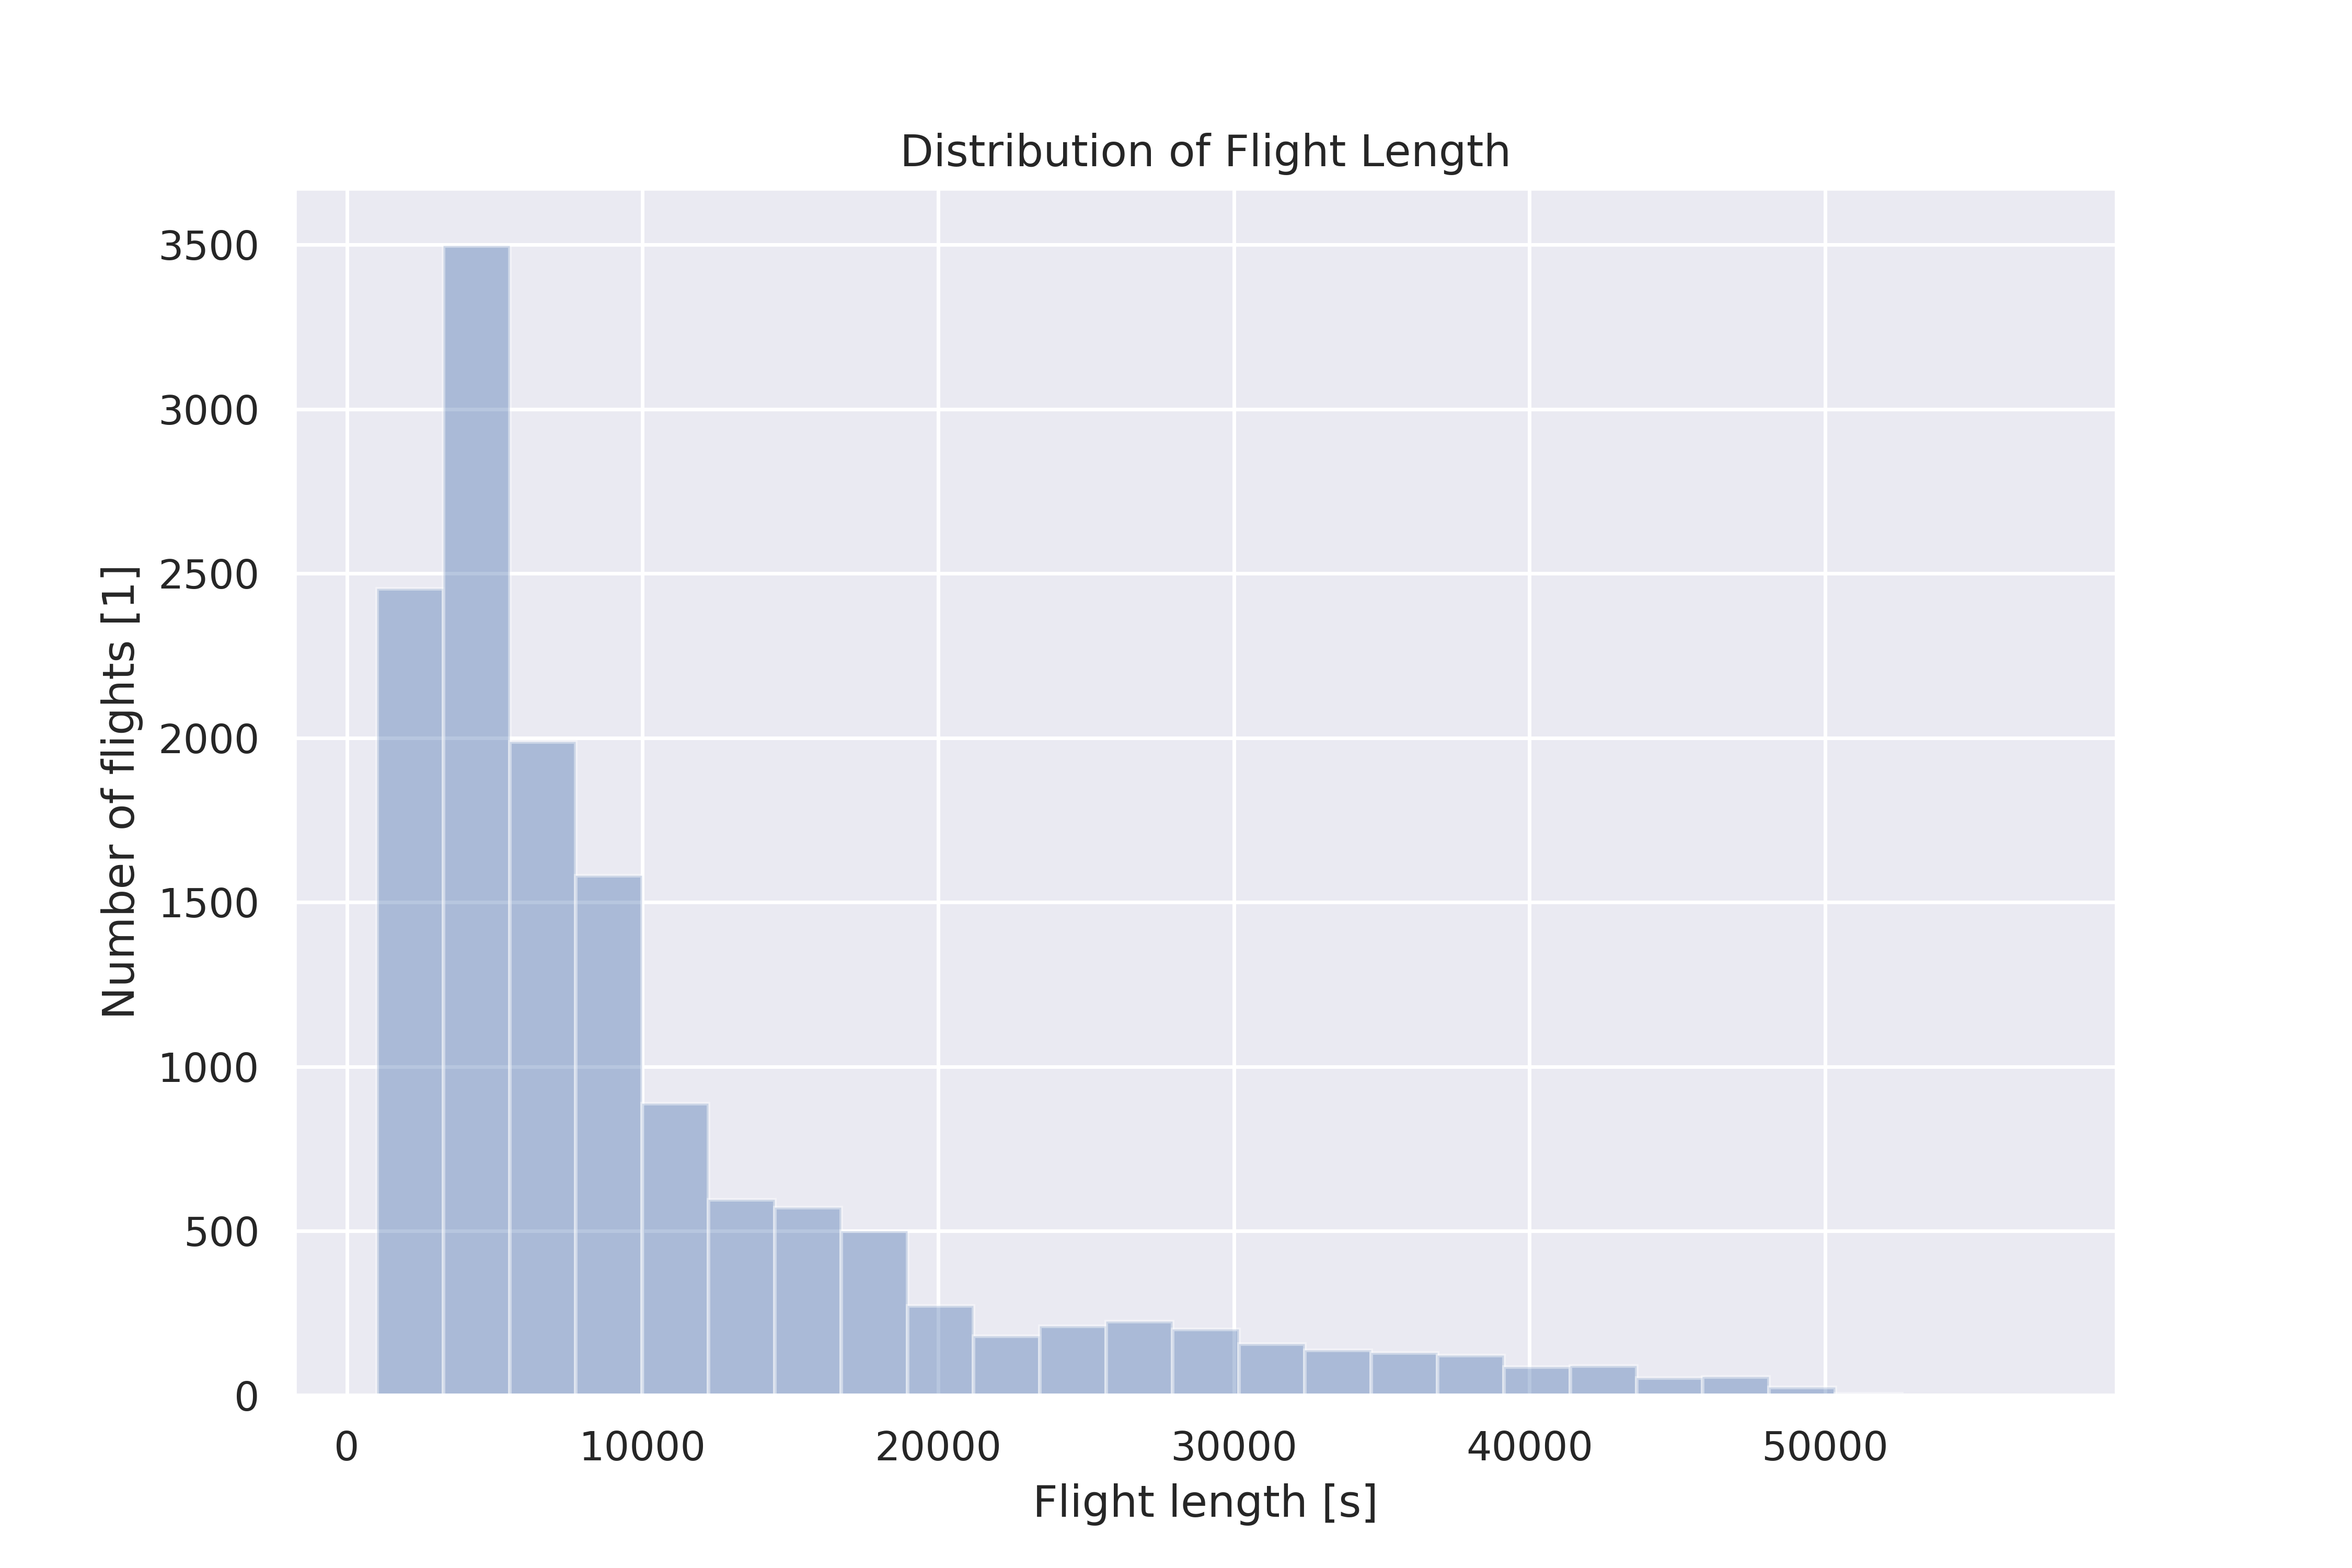
\includegraphics[width=0.8\textwidth]{length_hist}
    \caption{\label{fig:flt_len} A histogram of the lengths of 14045 flights}
\end{figure}

Each flight is represented by a CSV file with 216 columns, comprising one timestamp and 215 values per second of recording time.

The four flight parameters extracted were altitude (ALT), rotational speed of the high-pressure shaft (NH), and pressure and temperature of air exiting the compressor (P30 and T30, respectively). These are shown for one typical flight in Figure \ref{fig:flt_example}.



\subsection{Flight Phases}
Each flight can be split into several phases: preflight, taxi out, take-off, climb, cruise, descent, reverse thrust and taxi in.


\begin{figure}
    \centering
    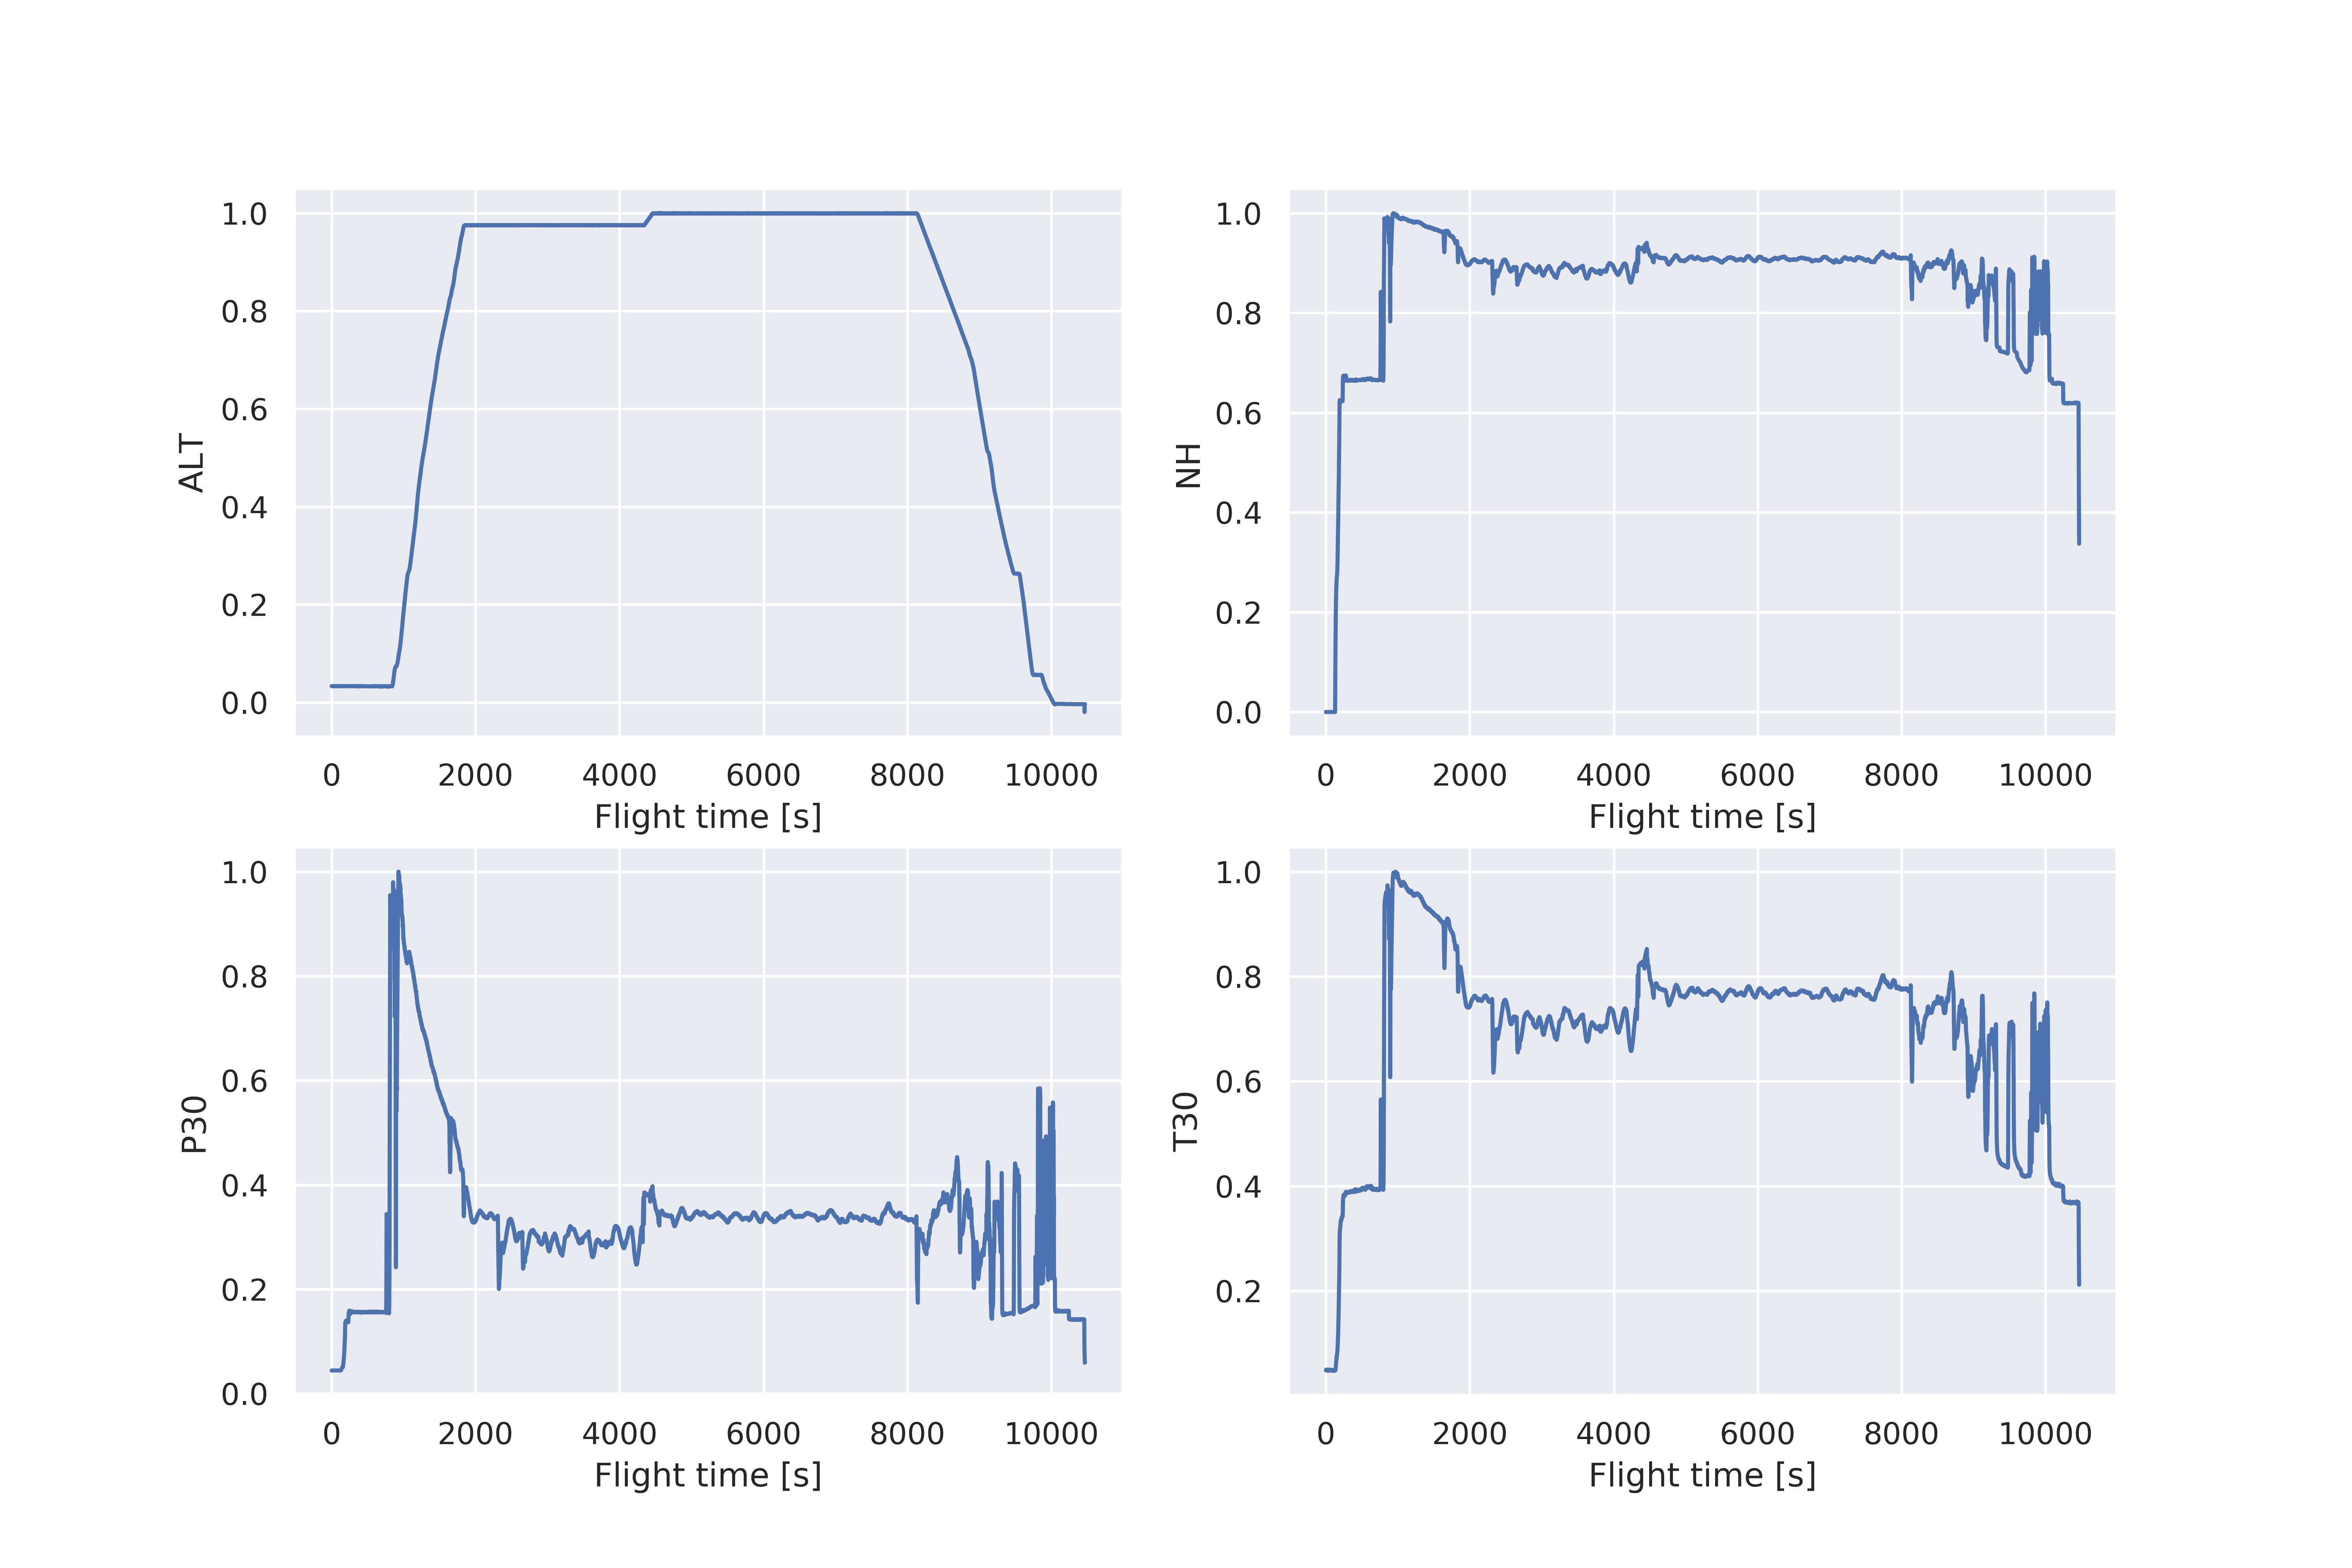
\includegraphics[width=0.8\textwidth]{6008_20150409074414}
    \caption{\label{fig:flt_example} ALT, NH, P30 and T30 of a randomly selected flight. All parameter values are normalised.}
\end{figure}


\subsection{Output}
The flights were processed using SA66 (Section \ref{sa66}) to determine the number of cycles consumed

\subsubsection{Cycle Counter}

\subsection{Visualisation}

\subsection{Downsampling}

\subsubsection{(A)PLA}

\subsubsection{APCA}

\subsection{Case Studies}

\subsubsection{6014: Stress Ranges}

\subsubsection{6079: Long Taxi}